\documentclass[12pt,a4paper]{article}
\usepackage{float}
\usepackage{graphicx}
\usepackage{minted}

\title{UE23CS343AB2 Lab 2}
\author{Aditya Hegde \@- PES2UG23CS032}
\date{\today}

\begin{document}
\maketitle

\section{Hadoop Installation}
\subsection{Installation Assertion and Startup}

\begin{figure}[H]
   \centering
   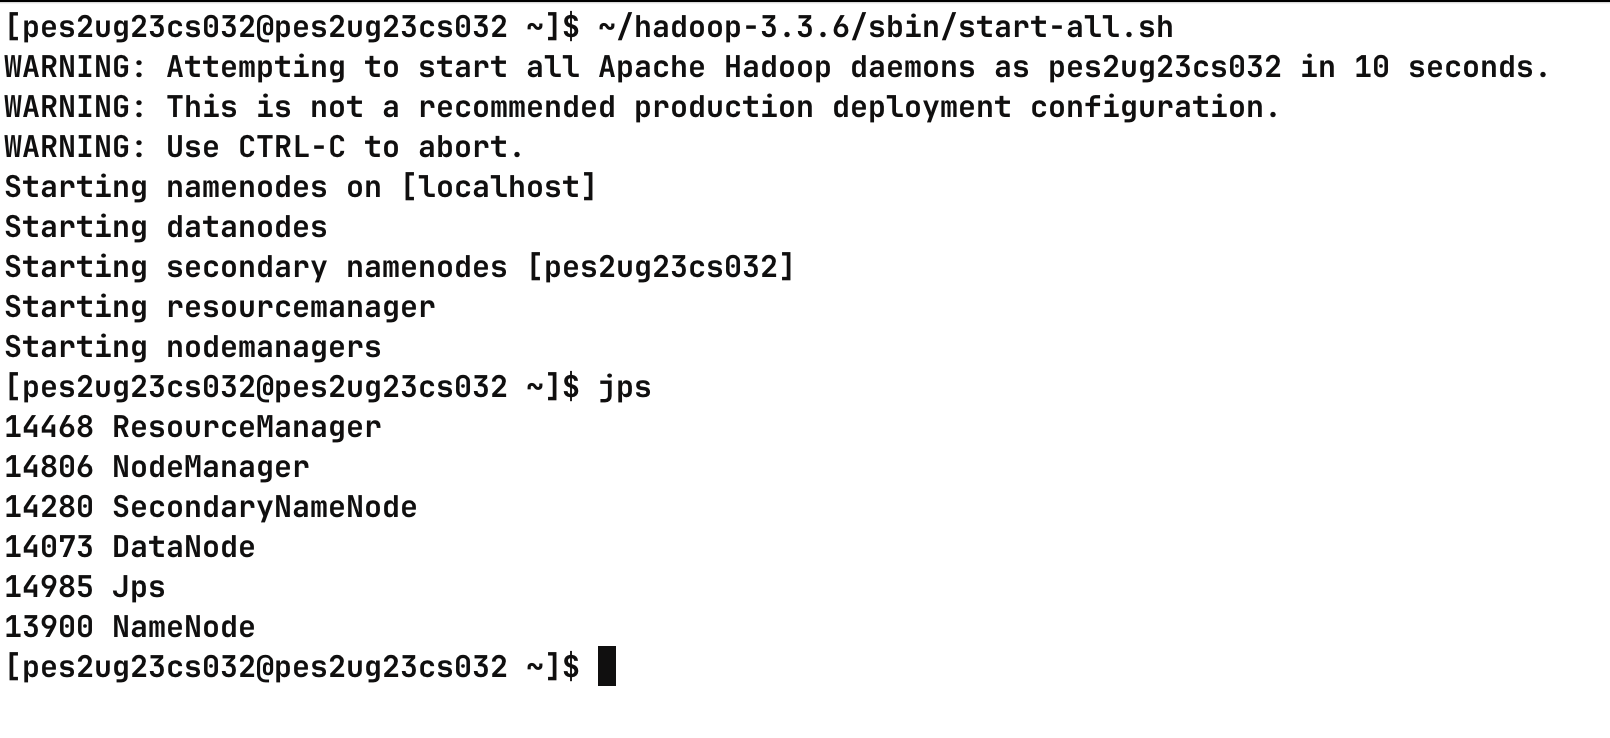
\includegraphics[width=0.8\textwidth]{./images/img1.png} 
   \caption{Hadoop Startup and \texttt{jps} command output}
\end{figure}

\subsection{HDFS \texttt{dfs} tests}
\begin{figure}[H]
    \centering
    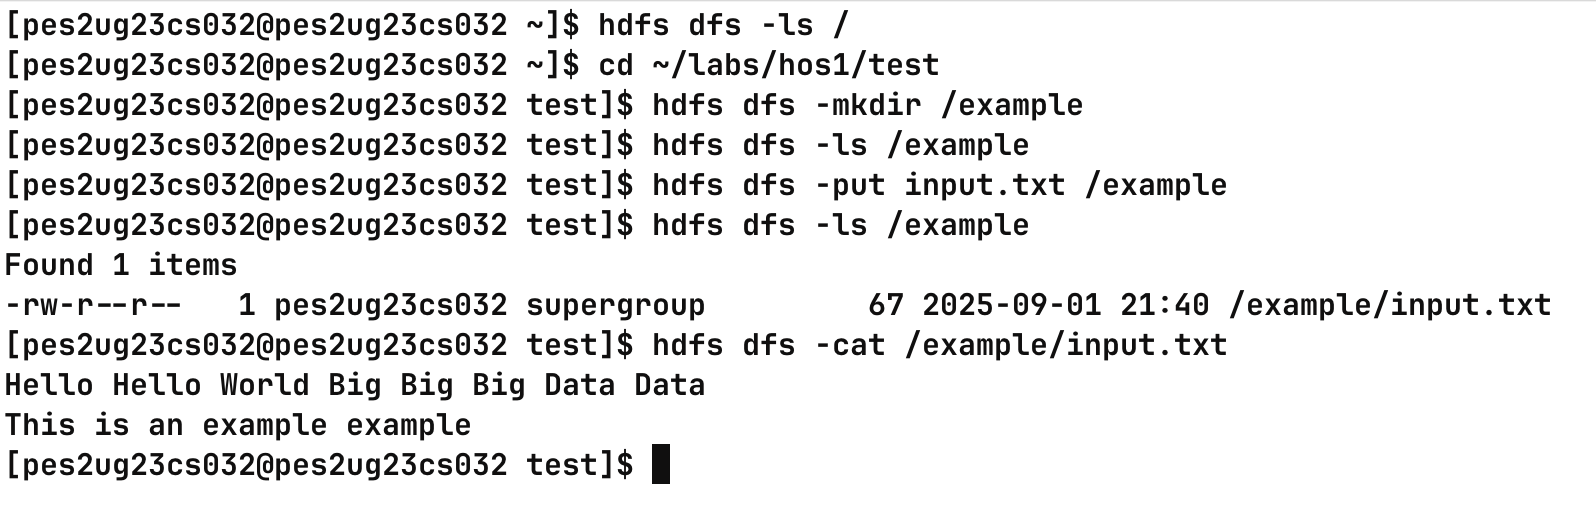
\includegraphics[width=0.7\textwidth]{./images/img2.png}
    \caption{Uploading a file to HDFS}
\end{figure}

\subsection{Running map-reduce example \texttt{jar}}
\begin{figure}[H]
    \centering
    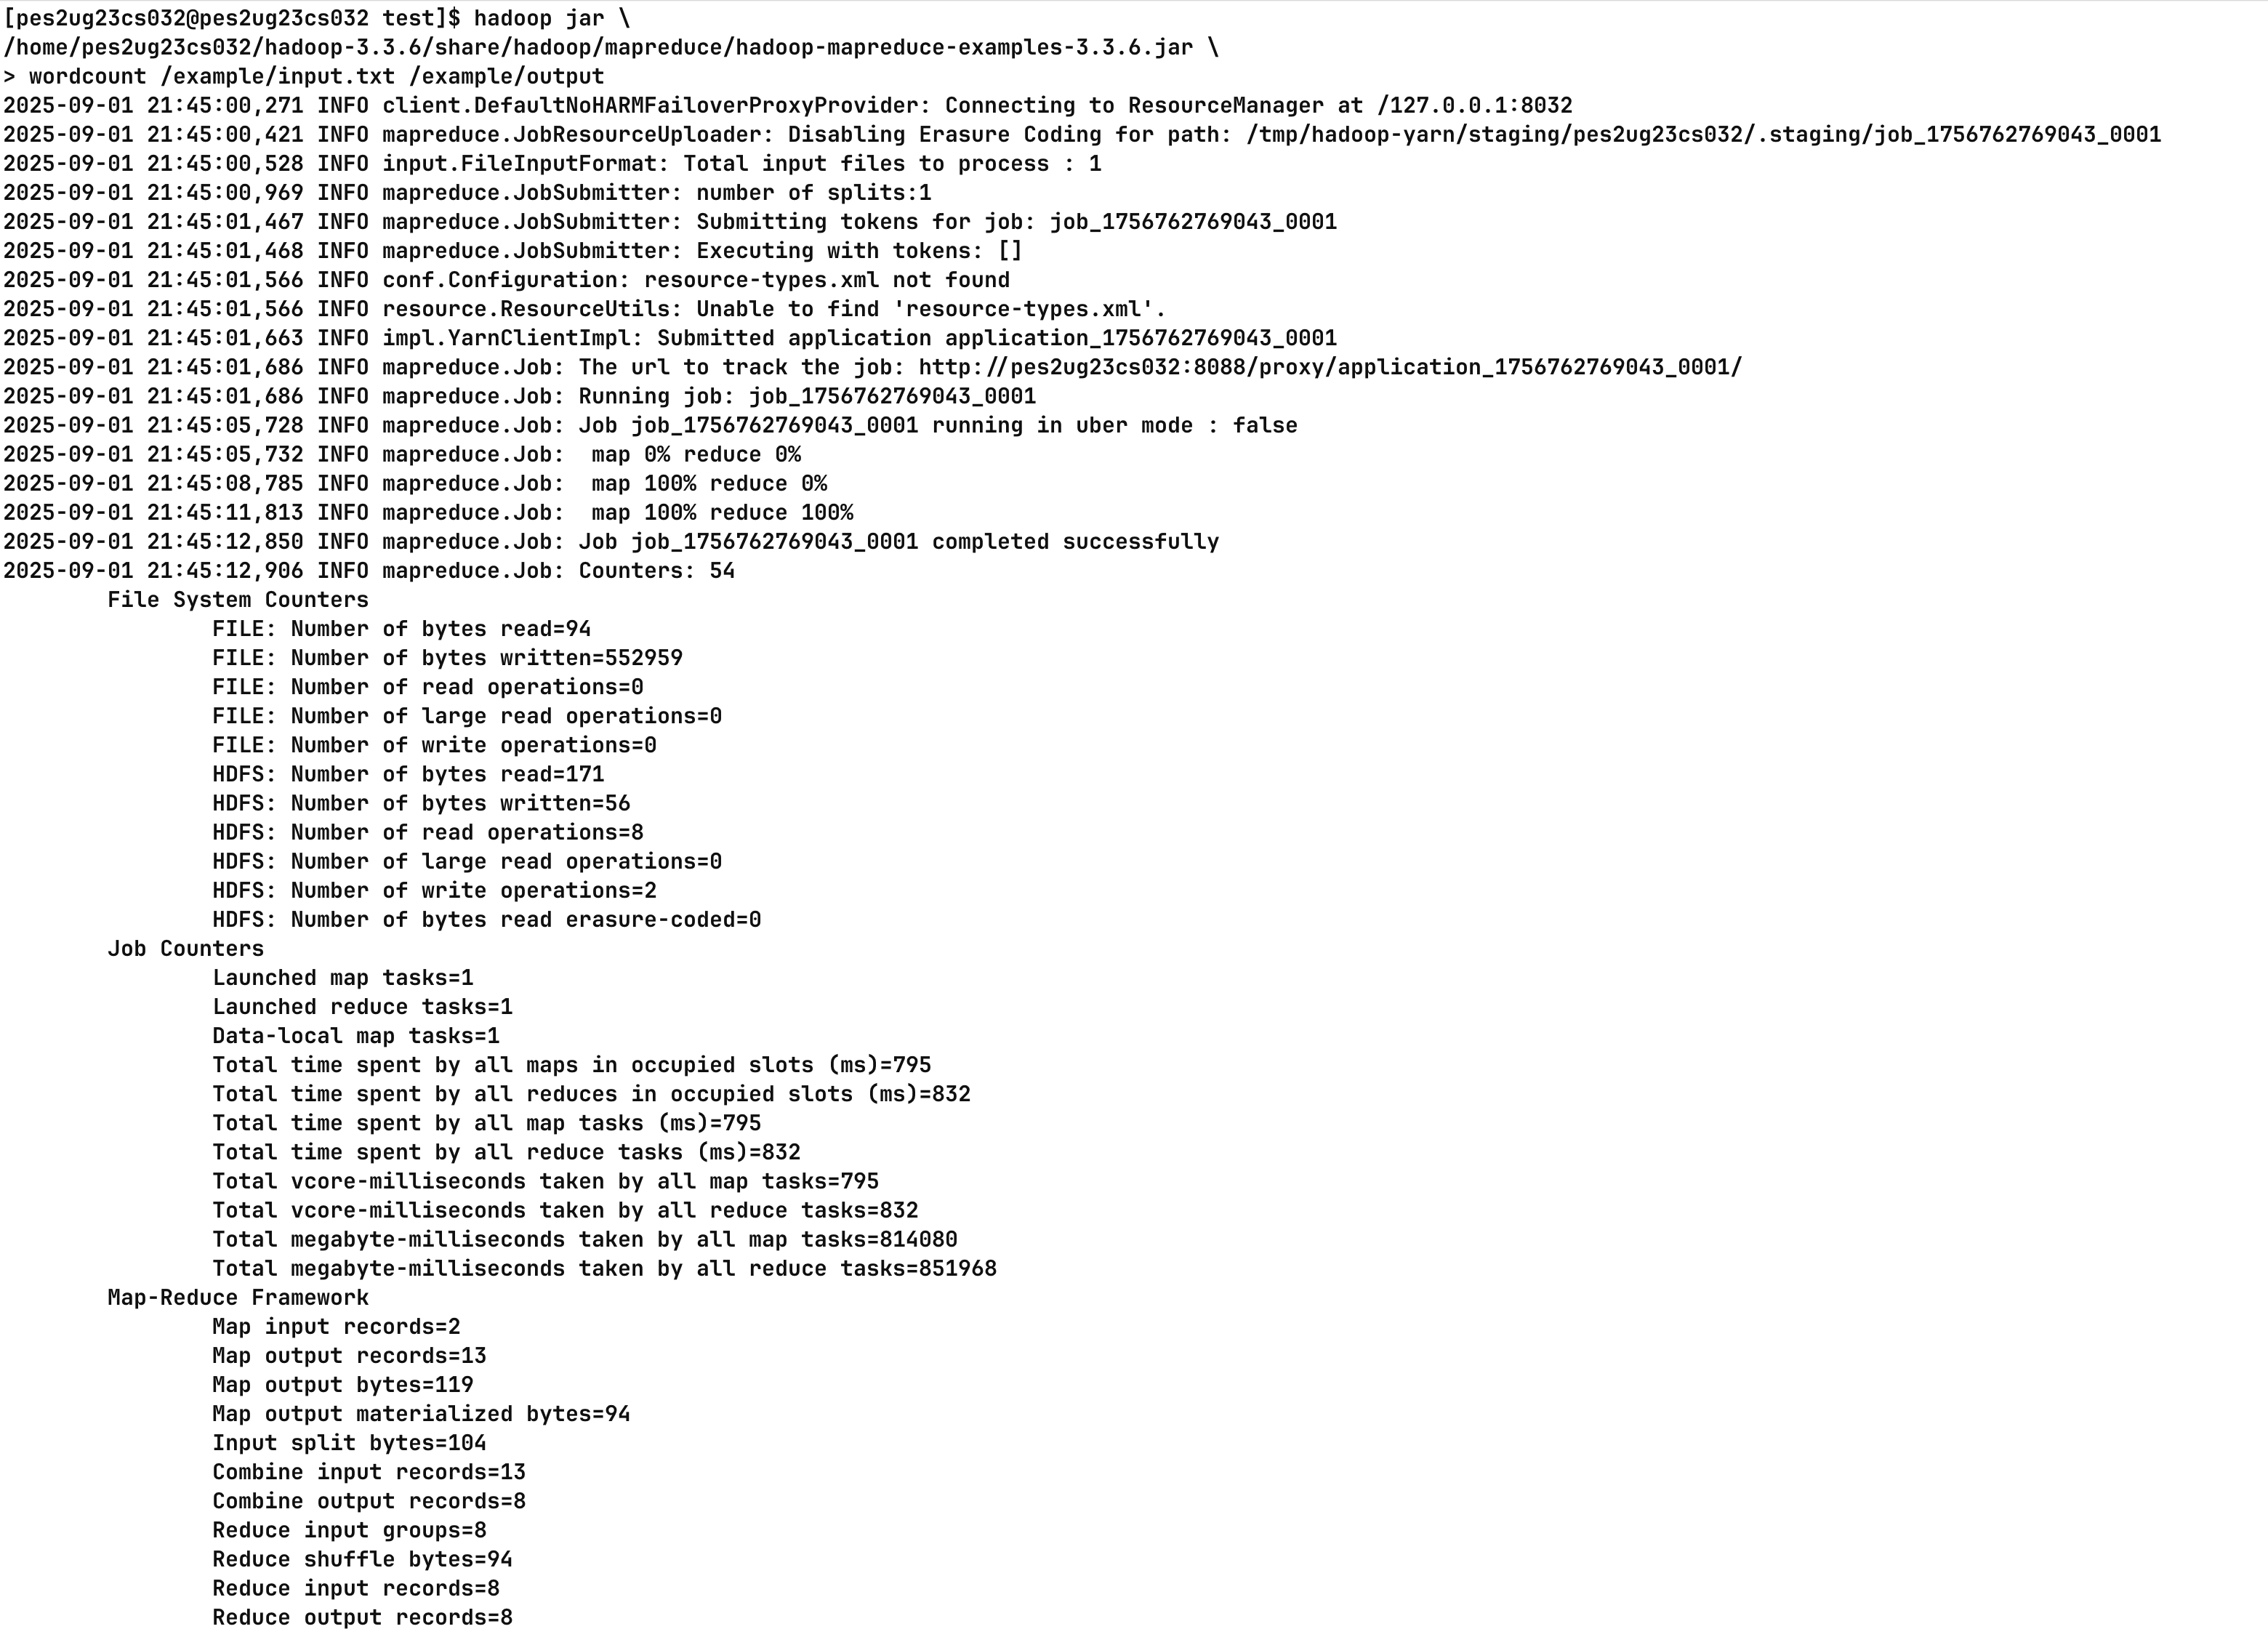
\includegraphics[width=\textwidth]{./images/img3.png}
\end{figure}

\begin{figure}[H]
    \centering
    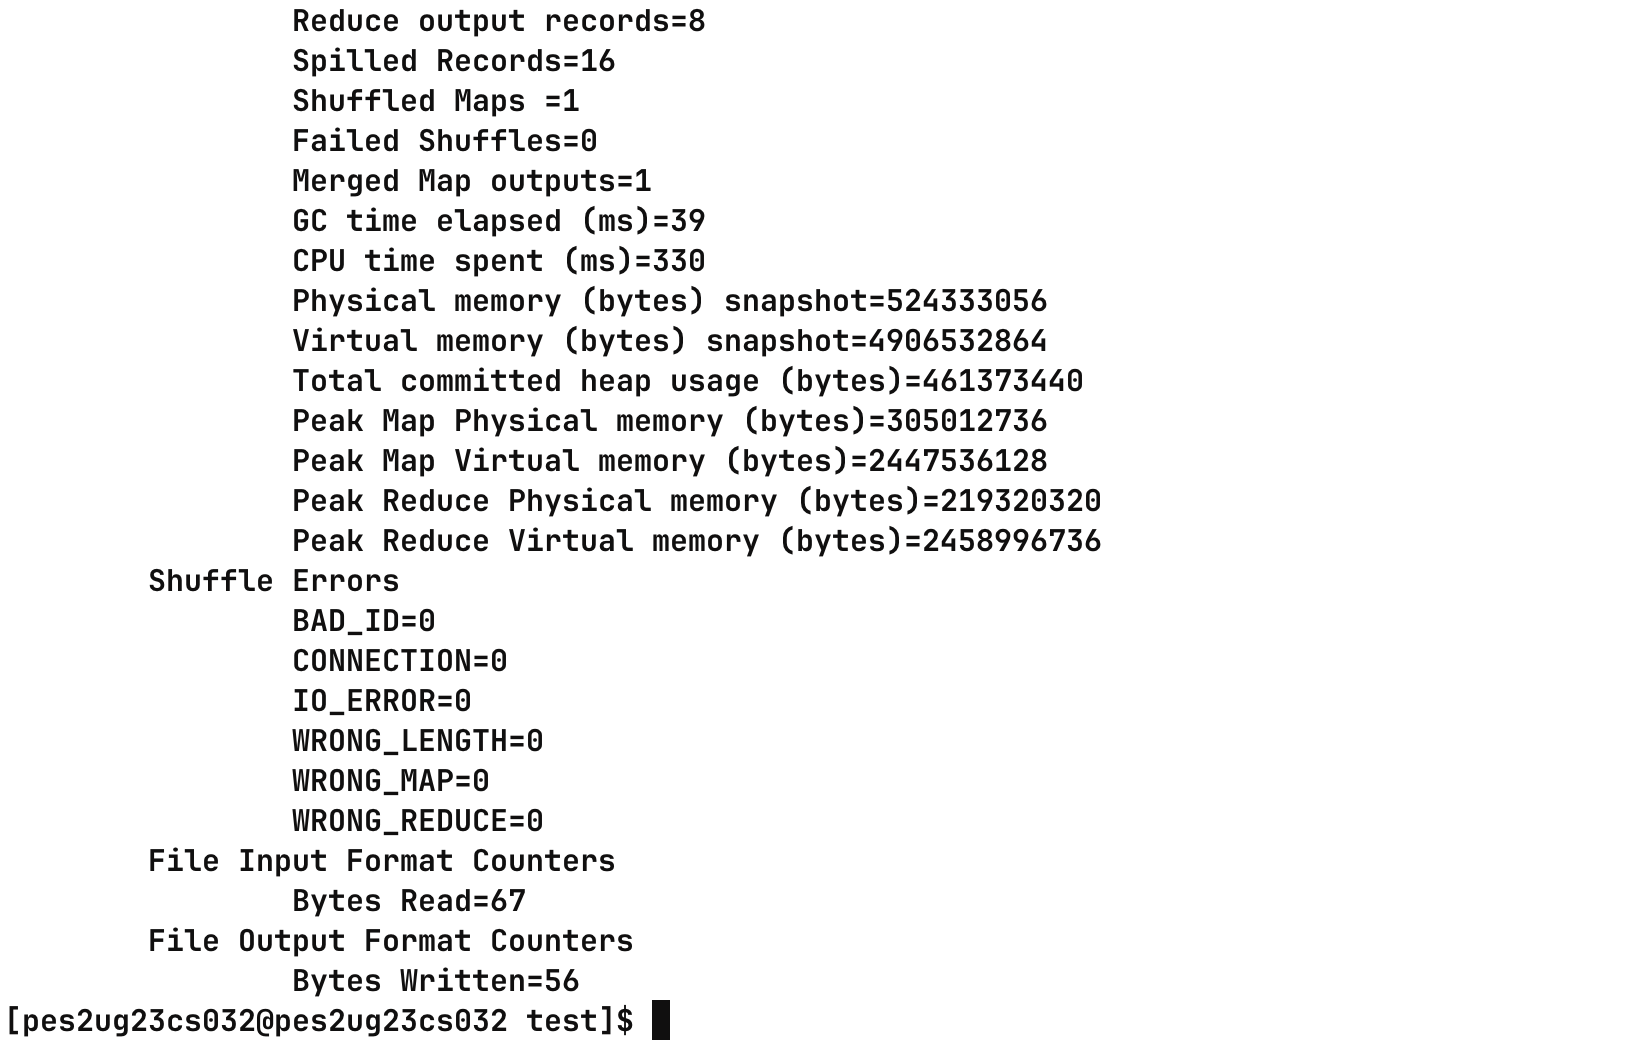
\includegraphics[width=0.8\textwidth]{./images/img3b.png}
    \caption{Example hadoop map-reduce wordcount jar}
\end{figure}

\begin{figure}[H]
   \centering
   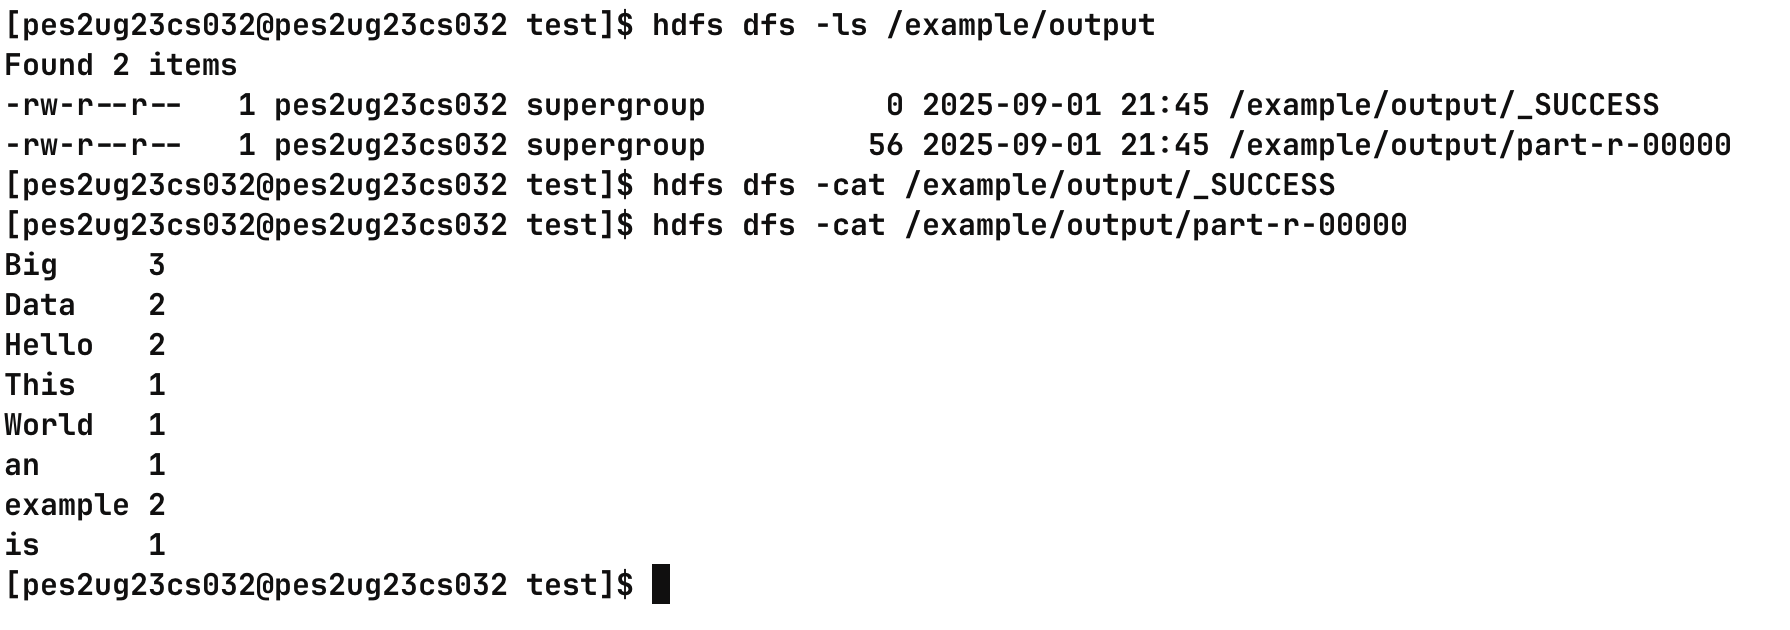
\includegraphics[width=0.8\textwidth]{./images/img4.png} 
   \caption{Example hadoop map-reduce wordcount output}
\end{figure}

\section{Simulating Map Reduce}

\begin{figure}[H]
\centering
\begin{minted}{python}
#!/usr/bin/env python3

import sys

for line in sys.stdin:
    words = line.split()
    for word in words:
        print(f"{word},1")
\end{minted}
\caption{Python mapper script for word count}
\end{figure}

\begin{figure}[H]
\centering
\begin{minted}{python}
#!/usr/bin/env python3
import sys

prev_word = None
count = 0

for line in sys.stdin:
        curr_word, value = line.split(",")
        value = int(value)
        if(curr_word == prev_word):
                count += value
        else:
                if prev_word:
                        print(prev_word,count)
                count = 1
        prev_word = curr_word

print(prev_word,count)
\end{minted}
\caption{Python reducer script}
\end{figure}

\begin{figure}[H]
   \centering
   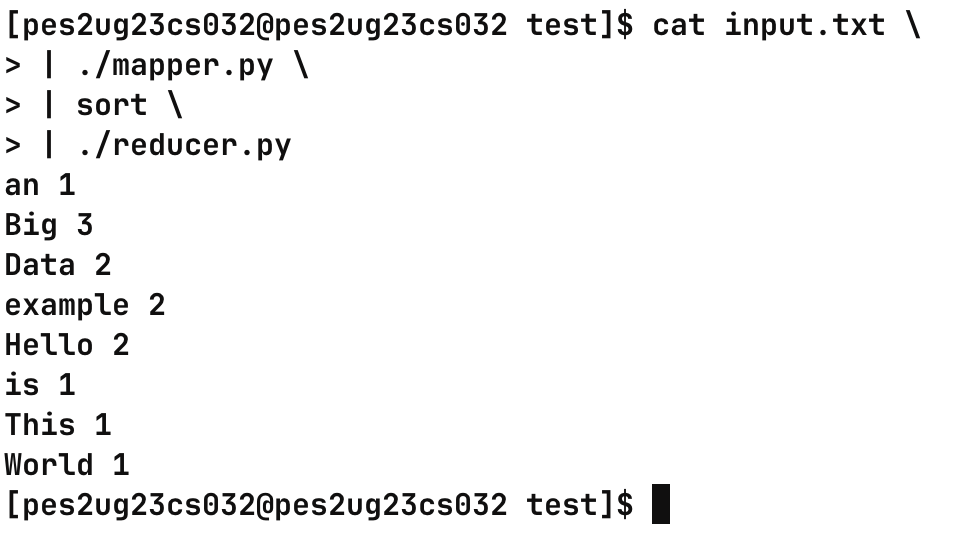
\includegraphics[width=0.8\textwidth]{./images/img5.png} 
   \caption{Simulated map-reduce word count output}
\end{figure}

\section{Example Movies Rating Dataset}

\begin{figure}[H]
   \centering
   \begin{minted}{python3}
#!/usr/bin/env python3

import sys

_ = list(
    map(
        lambda line: print(f"{line[0]}\t{int(line[1])}"),
        map(lambda x: x.strip().split(","), sys.stdin),
    )
)
   \end{minted}
   \caption{Mapper script for parsing movie ratings}
\end{figure}

\begin{figure}[H]
   \centering
   \begin{minted}{python3}
#!/usr/bin/env python3

import sys
from itertools import groupby, tee
from operator import itemgetter
from functools import reduce

parsed = map(
    lambda line: (line[0], float(line[1])),
    map(lambda x: x.strip().split("\t"), sys.stdin),
)

for movie, group in groupby(parsed, key=itemgetter(0)):
    total, count = reduce(
        lambda acc, x: (acc[0] + x, acc[1] + 1), 
        map(itemgetter(1), group), 
        (0.0, 0)
    )
    print(f"{movie}\t{total / count}")
   \end{minted}
   \caption{Reducer script for movie ratings average}
\end{figure}

\begin{figure}[H]
   \centering
   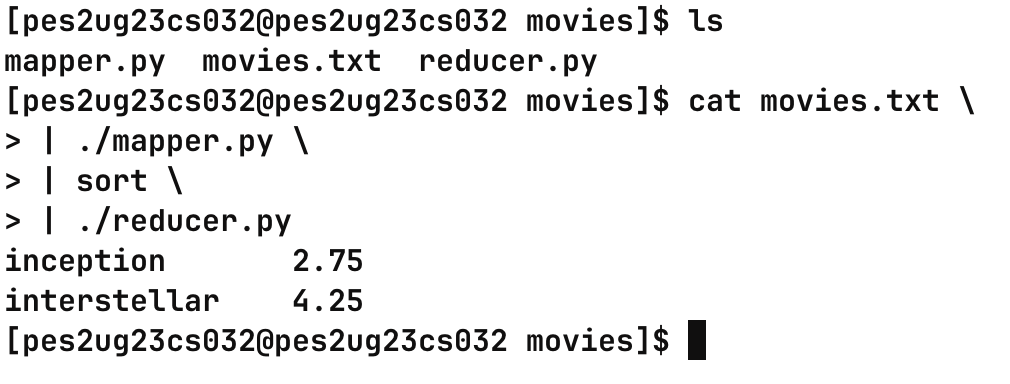
\includegraphics[width=0.8\textwidth]{./images/img6.png} 
   \caption{Simulated map-reduce word count output}
\end{figure}

\end{document}